%!TEX TS-program = xelatex
%!TEX encoding = UTF-8 Unicode

\documentclass[nols,b5paper]{tufte-book}

\usepackage{booktabs}
\usepackage{graphicx}
\usepackage{listings}

\usepackage{mathspec}
\usepackage{fontspec,xltxtra,xunicode}
\defaultfontfeatures{Mapping=tex-text}
\setromanfont[Mapping=tex-text]{Chaparral Pro}
\setsansfont[Scale=MatchLowercase,Mapping=tex-text]{Frutiger LT Std}
\setmonofont[Scale=MatchLowercase]{Andale Mono}
\setmathfont(Greek,Latin,Digits){Chaparral Pro}

\graphicspath{{./figures/}}

\usepackage{color}
\lstset{ %
language=Python,                % the language of the code
numbers=left,                   % where to put the line-numbers
stepnumber=2,
numbersep=5pt,                  % how far the line-numbers are from the code
backgroundcolor=\color{white},  % choose the background color. You must add 
showspaces=false,               % show spaces adding particular underscores
showstringspaces=false,         % underline spaces within strings
showtabs=false,                 % show tabs within strings adding particular underscores
frame=single,                   % adds a frame around the code
tabsize=2,                      % sets default tabsize to 2 spaces
breaklines=true                % sets automatic line breaking
}

\title{bipy -- documentation}
\author[\textsc{bipy user manual}]{Timothée Poisot}
\date{Version pre 1.0}

\begin{document}

\maketitle
\tableofcontents

\chapter{Introduction}

\texttt{bipy} is a set of functions written in Python, whose goal is to make it easy to analyze and visualize bipartite networks. This document describes the use of the \texttt{bipy}. This documentation is valid only for the versions before the 1.0 release (scheduled to occur sometime in the fall or winter of 2011). The aim of this documentation is to present only the ``high-level'' functions, i.e. these that the user will need to perform the analyses (although \texttt{bipy} was conceived to automate most of the analyses, so there are a very small number of functions that need to be known). In addition, some background about the measures used and the most important references will be given.

\subsection{Installing \texttt{bipy}}

\texttt{bipy} can be obtained on \emph{GitHub} (http://github.com/tpoisot/bipy). There are a number of required additional software. Obviously, \texttt{bipy} requires a Python installation, preferentially 2.6 or 2.7. For those of you with a Mac, you need to download the version from python.org (http://www.python.org/getit/).

Once this is done, 

\subsection{Do I need to know Python ?}

This is a good question! If you just want to have basic informations about your data, the short answer is \textbf{no}. \texttt{bipy} was designed from the beginning to automate most of the calculations, and use the most robust statistics available, so you don't have to play too much with the code. Most of what you will have to do is start python, load your data, and use the summary functions.

If you want to use \texttt{bipy} for more complicated analyses, then \textbf{yes}, learning python will definitely be a huge plus. But if you are willing to adopt a computational approach, chances are you already know a programming language, and you should be able to pick up python really quick.

\chapter{Loading data}

This chapter describes how to load data in a format that can be understood by \texttt{bipy}. There are two different ways to load data in \texttt{bipy}: \emph{via} a text file, or \emph{via} the web \footnote{Actually, there exists a third way to load data, namely the interaction with the \textsc{ewdb} -- given that this database is still highly experimental, and that the server on which it is developed is not ready to support real usage, this will be introduced in future versions of \texttt{bipy}. }. We will cover both in this chapter.

\subsection{Reading data from a local file}

Most of the time, this will be the default solution. \texttt{bipy} assumes that a bipartite network is nothing more than a matrix, in which each square represents the strength of the interaction between a species from the top trophic level, and a species from the bottom trophic level. Thus, a bipartite network is defined by a matrix $\mathbf{M}$, in which $\mathbf{M}\sb{ij}$ is the strength of the link between upper trophic level species $i$ and lower trophic level species $j$. It is assumed that the rows of $\mathbf{M}$ are the upper trophic level species. This is a notational convention, but we will stick to it through all the documentation.

The advantage of this organization of the data is that it can easily be stored in a text file, with each interaction strength separated by a space, and the different organisms separated by a new line. Thus, the file

\begin{marginfigure}[3cm]
	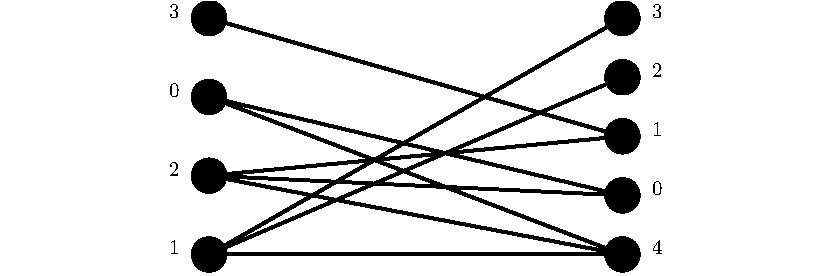
\includegraphics[width=4.5cm]{ex-1}
\end{marginfigure}

\begin{verbatim}
1 0 0 0 1
0 0 1 1 1
1 1 0 0 1
0 1 0 0 0
\end{verbatim}

\noindent described the network illustrated in the margin. Of course, the values within the file can be anything (as long as they are numeric): zeroes and ones, number of visits, predation rate, percent of the diet, and so on.

Assuming that your data are in this format, and the file is called \texttt{mydata.web}, you can load them with

\begin{lstlisting}
web = readweb('mydata.web')
\end{lstlisting}

This will only create a 2-dimensional array. The power of \texttt{bipy} lies in its ability to automate the calculations, so it is better to write

\begin{lstlisting}
web = bipartite(readweb('mydata.web'))
\end{lstlisting}

Most of the functions will need an object returned by the \texttt{bipartite} function, so it is good practice to use it \footnote{The actual reason is that most of the networks statistics will need simple informations, such as number of links per species, connectance, size of the network. The \texttt{bipartite} class calculate all of them once and for all, so this avoid re-calculating the same information several times.}. At this point, the most difficult part is done. Your data are loaded, and you will be able to see what story they tell using the metrics described in the other chapters.

If your data are not in the ``correct'' format, i.e. the top level organisms are in columns, do not panic. You just need to pass a supplementary argument \texttt{t} to the \texttt{bipartite} function:

\begin{lstlisting}
web = bipartite(readweb('mydata.web'),t=True)
\end{lstlisting}

This will the the \texttt{bipy}	 that your data need to be transposed before going on with the analysis.

\subsection{Reading data from the web}

The alternative way is to load data stored on the internet. \texttt{bipy} is able to do so by using the \texttt{readRemoteWeb} function, which requires three arguments. The first one is the \textsc{url} of a text file, which stores the interaction matrix. The second are two booleans, telling if the network should be transformed using \texttt{bipartite} (true by default), and if the network should be transposed (false by default).

\begin{lstlisting}
web = readRemoteWeb('http://server/mydata.web'),True,False)
\end{lstlisting}

\subsection{Adding species names}

\subsection{Adding bibliographical references}

\chapter{Species--level metrics}

\chapter{Network--level metrics}

\chapter{Null models}

\chapter{Graphics}

\chapter{Example scripts}

\end{document}